\documentclass[9pt]{article}
\usepackage[english]{babel}
\usepackage{amsmath,amsthm}
\usepackage{amsfonts}
\usepackage{graphicx}
\usepackage[margin=0.2in]{geometry}
\newcommand{\setlinespacing}[1]{\setlength{\baselineskip}{#1 \defbaselineskip}}
\newcommand{\doublespacing}{\setlength{\baselineskip}{2.0 \defbaselineskip}}
\newcommand{\singlespacing}{\setlength{\baselineskip}{\defbaselineskip}}
\newcommand{\A}{{\cal A}}
\newcommand{\h}{{\cal H}}
\newcommand{\s}{{\cal S}}
\newcommand{\W}{{\cal W}}
\newcommand{\BH}{\mathbf B(\cal H)}
\newcommand{\KH}{\cal  K(\cal H)}
\newcommand{\Real}{\mathbb R}
\newcommand{\Complex}{\mathbb C}
\newcommand{\Field}{\mathbb F}
\newcommand{\RPlus}{[0,\infty)}
\newcommand{\norm}[1]{\left\Vert#1\right\Vert}
\newcommand{\essnorm}[1]{\norm{#1}_{\text{\rm\normalshape ess}}}
\newcommand{\abs}[1]{\left\vert#1\right\vert}
\newcommand{\set}[1]{\left\{#1\right\}}
\newcommand{\seq}[1]{\left<#1\right>}
\newcommand{\eps}{\varepsilon}
\newcommand{\To}{\longrightarrow}
\newcommand{\RE}{\operatorname{Re}}
\newcommand{\IM}{\operatorname{Im}}
\newcommand{\Poly}{{\cal{P}}(E)}
\newcommand{\EssD}{{\cal{D}}}
\newcommand{\field}[1]{\mathbb{#1}}
\newcommand{\C}{\field{C}}
\newcommand{\R}{\field{R}}
\newcommand{\script}[1]{\mathcal{#1}}
\newcommand{\fall}{\; \forall \;}
\newcommand{\exts}{\; \exists \;}
\newcommand{\mbf}[1]{\mathbf{#1}}
\newcommand{\binomial}[2]{\biggl( \begin{array}{c}  #1 \\ #2  \\ \end{array} \biggr) }
\newcommand{\fderiv}[2]{ \frac{d}{ d #1} \: #2}
\newcommand{\sderiv}[2]{ \frac{d^2}{ d^2 #1} \: #2}
\newcommand{\pfderiv}[2]{ \frac{\partial}{ \partial #1} \: #2}
\newcommand{\psderiv}[2]{ \frac{\partial^2}{ \partial^2 #1} \: #2}
\newcommand{\mat}[1]{\mathbf{#1}}
\DeclareSymbolFont{AMSb}{U}{msb}{m}{n}
\DeclareMathSymbol{\dblz}{\mathalpha}{AMSb}{"5A}
\DeclareMathSymbol{\dblr}{\mathalpha}{AMSb}{"52}
\DeclareMathSymbol{\dblt}{\mathalpha}{AMSb}{"54}
\DeclareMathSymbol{\dblq}{\mathalpha}{AMSb}{"51}
\DeclareMathSymbol{\dbln}{\mathalpha}{AMSb}{"4E}
\DeclareMathSymbol{\dblf}{\mathalpha}{AMSb}{"46}
\DeclareMathSymbol{\dblc}{\mathalpha}{AMSb}{"43}
\DeclareMathSymbol{\dbld}{\mathalpha}{AMSb}{"44}
\theoremstyle{plain}
\newtheorem{thm}{Theorem}[section]
\newtheorem{cor}[thm]{Corollary}
\newtheorem{lem}[thm]{Lemma}
\newtheorem{prop}[thm]{Proposition}
\theoremstyle{definition}
\newtheorem{defn}{Definition}[section]
\theoremstyle{remark}
\newtheorem{rem}{Remark}[section]
\numberwithin{equation}{section}
\renewcommand{\theequation}{\thesection.\arabic{equation}}
\begin{document}
\title{Regression of KL Software Distribution   }
\author{KL Software Libraries}
\date{Tue May 13 20:05:54 2014
}
\maketitle
\textbf{ KL Library test output.  This LaTex file and the associated diagrams are produced by the KL software libraries.}
QueryPerformanceCounter  =  522.056
\subsubsection{Iterated Exponential Filtering }
$\mu_1 =0.0930085$
$\mu_2 =0.725636$
$\mu_3 =0.0110119$
$\mu_4 =2.17812$
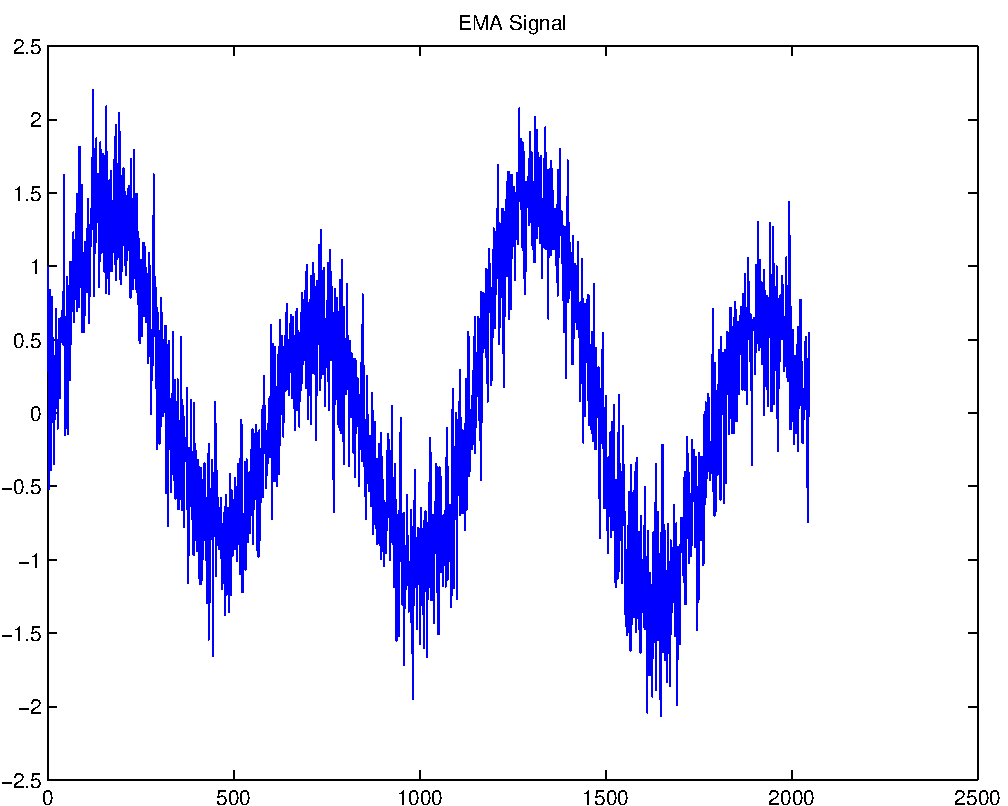
\includegraphics[width=10.0cm,height=10.0cm]{EMA_signal.pdf}

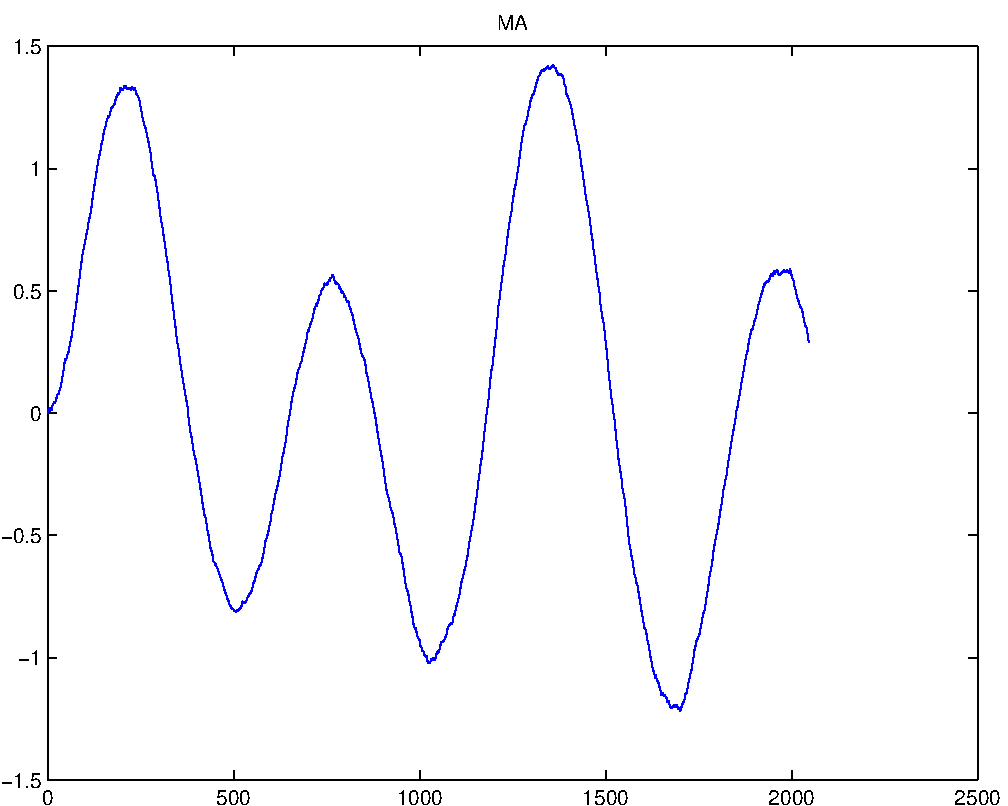
\includegraphics[width=10.0cm,height=10.0cm]{MA.pdf}

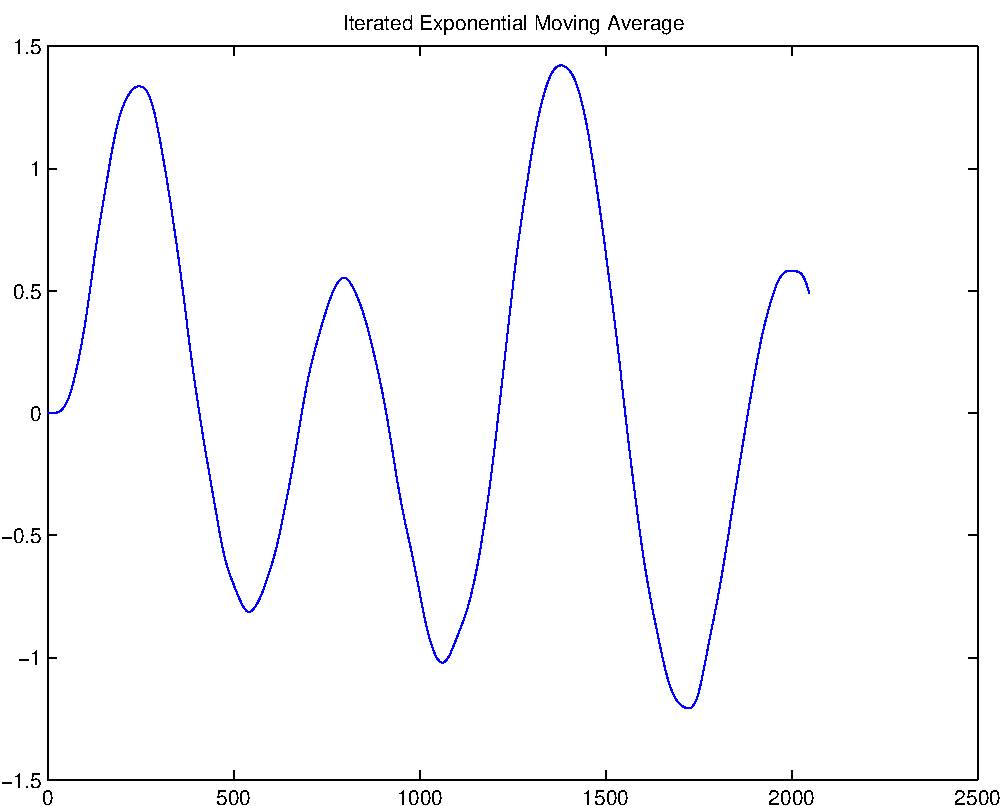
\includegraphics[width=10.0cm,height=10.0cm]{IEMA.pdf}

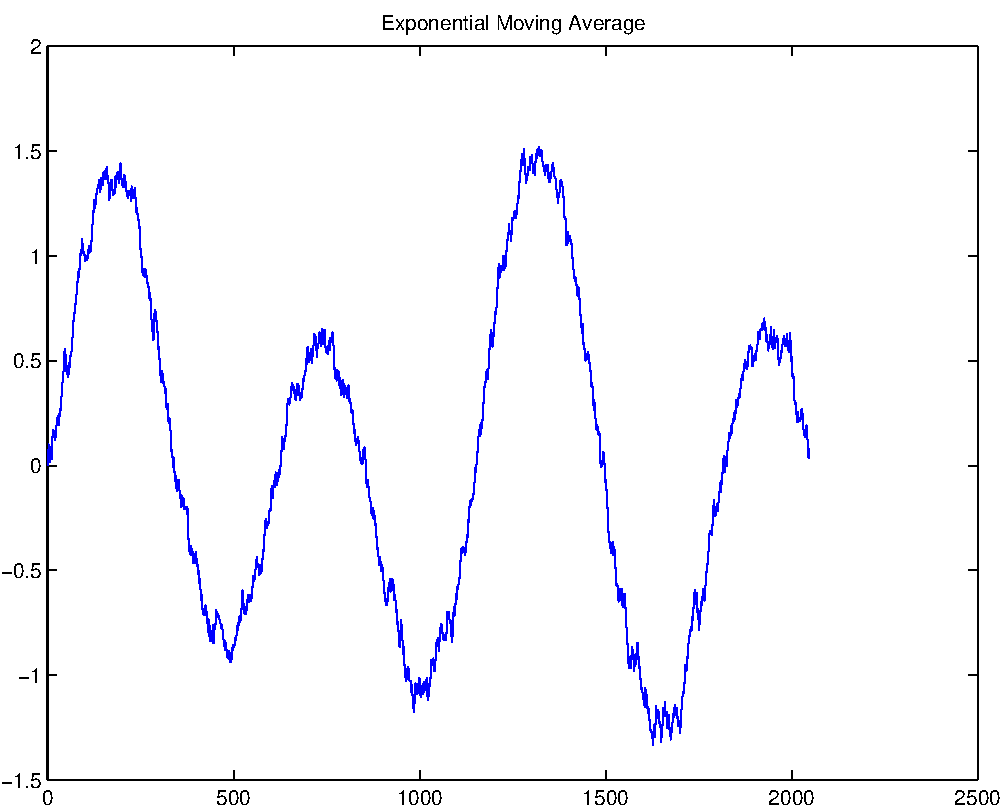
\includegraphics[width=10.0cm,height=10.0cm]{EMA.pdf}

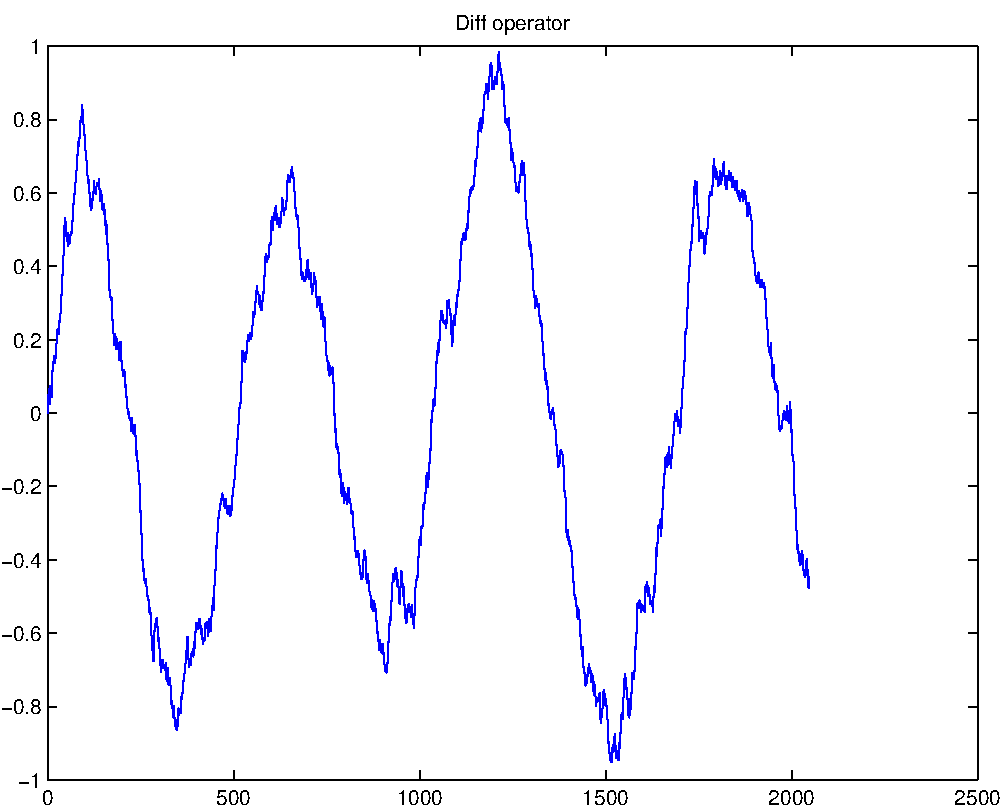
\includegraphics[width=10.0cm,height=10.0cm]{DIFF.pdf}

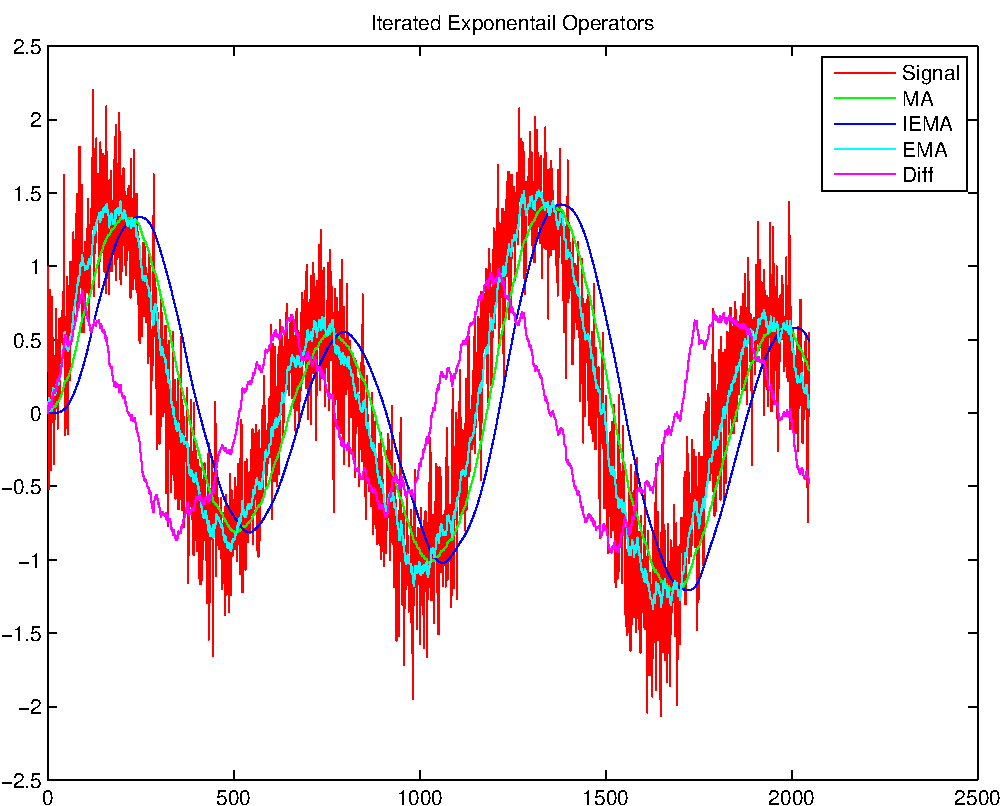
\includegraphics[width=10.0cm,height=10.0cm]{IteratedExponentailOperators.pdf}

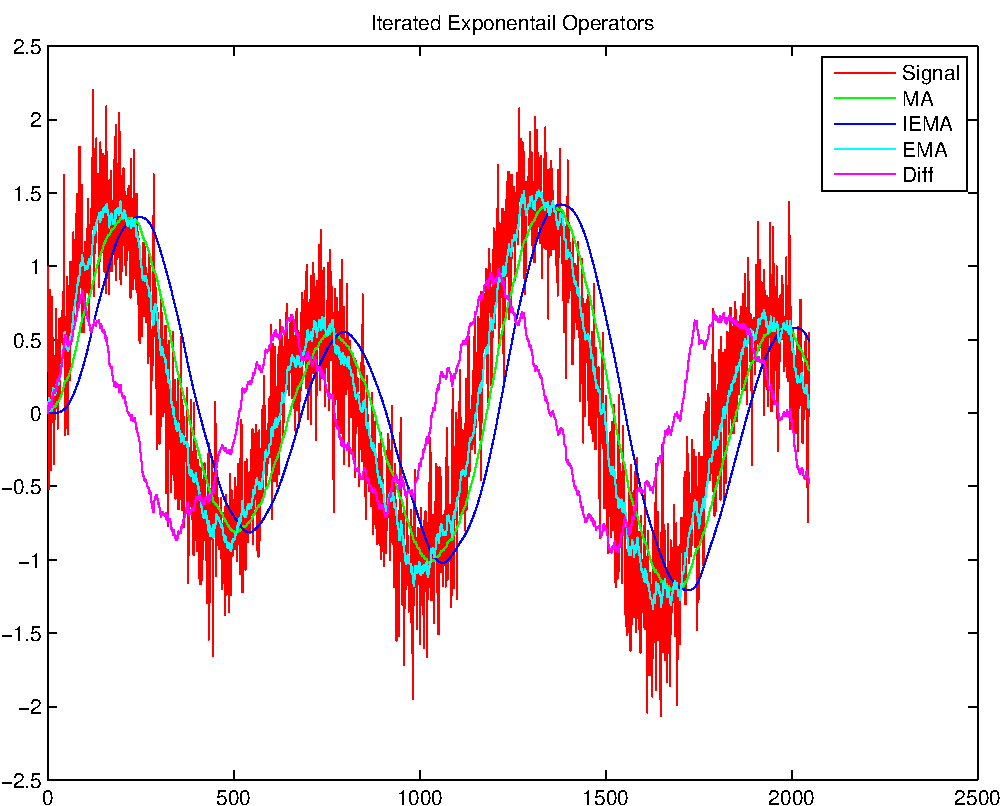
\includegraphics[width=10.0cm,height=10.0cm]{IteratedExponentailOperators.pdf}

QueryPerformanceCounter  =  9.02218
\subsubsection{Testing binary writer}
Binary writer Speedup 1GB Double Matrix 39.5086

Binary reader Speedup 1GB Double Matrix 1166.23

Binary writer Speedup 1GB Double vector 24.8827

Binary reader Speedup 1GB Double Matrix 936.523

QueryPerformanceCounter  =  3.22817
\subsubsection{Fast Gauss Transform}
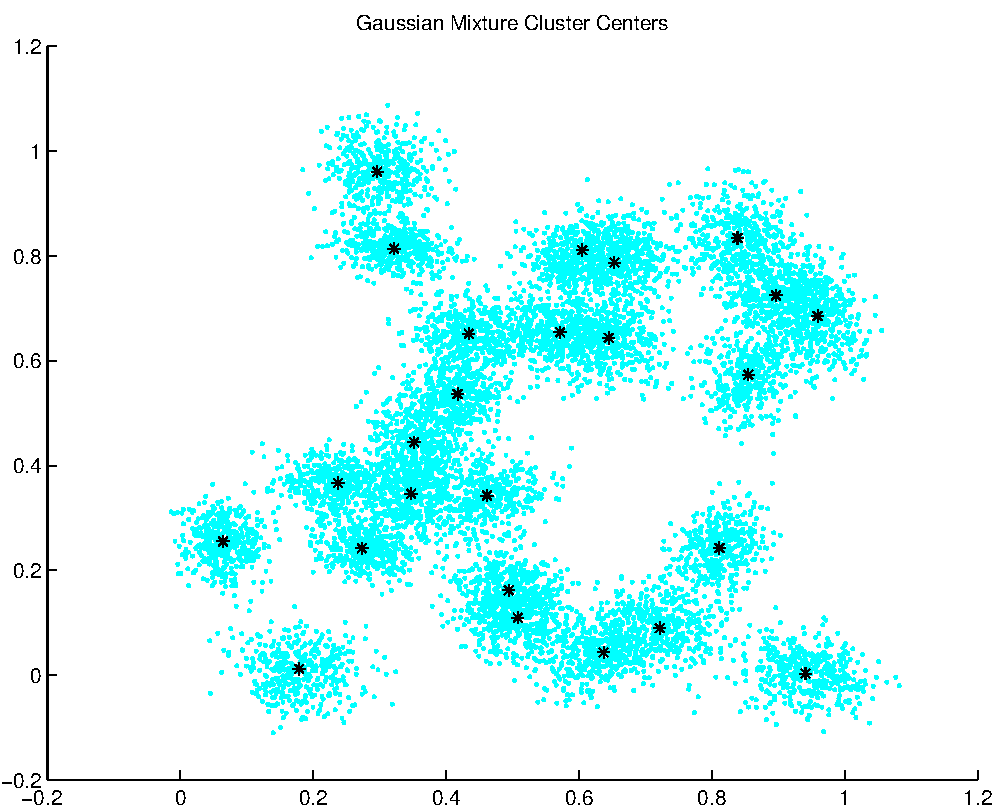
\includegraphics[width=10.0cm,height=10.0cm]{GaussianMixture_ClusterCenters25_Centers.pdf}

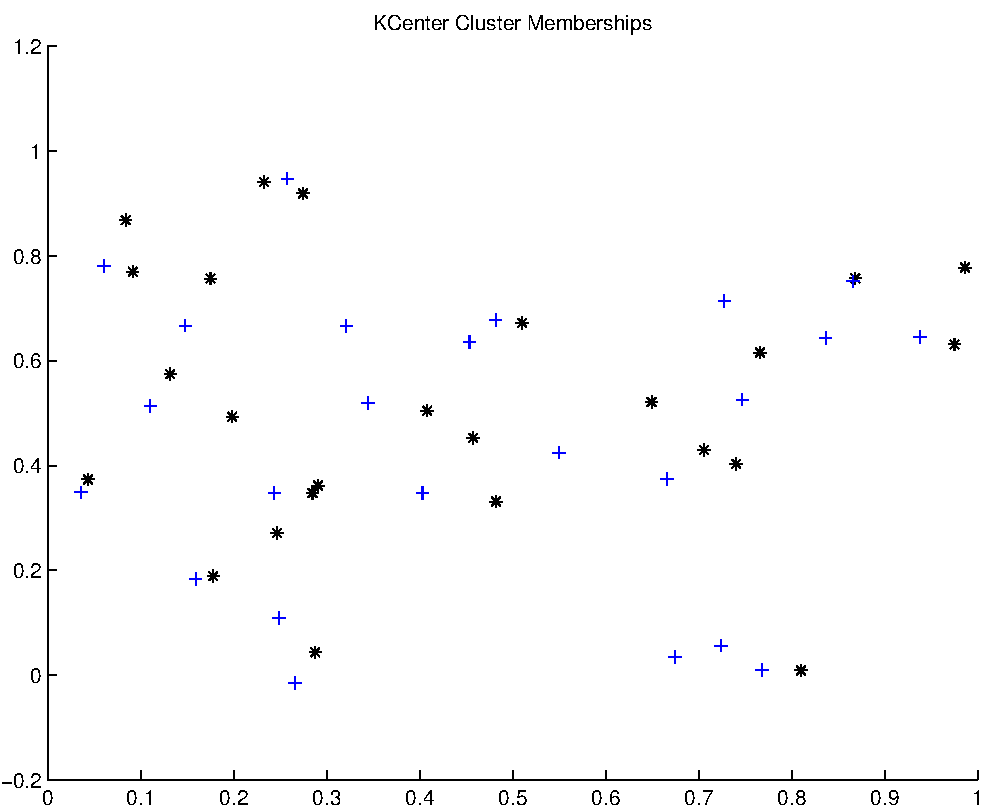
\includegraphics[width=10.0cm,height=10.0cm]{KCenterClusterMemberships_25_Centers.pdf}

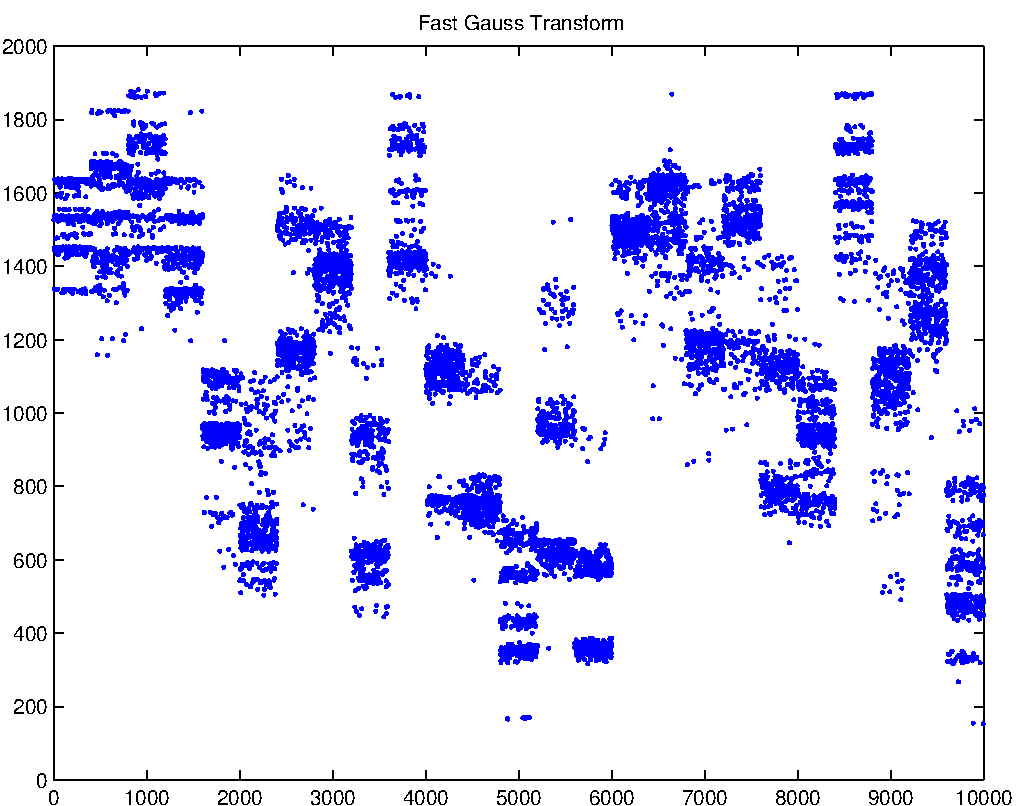
\includegraphics[width=10.0cm,height=10.0cm]{FGT25_Centers.pdf}

QueryPerformanceCounter  =  8.89701
\subsubsection{Testing Gaussian Mixture Point Cloud and Latex Plotting Capabilities.}
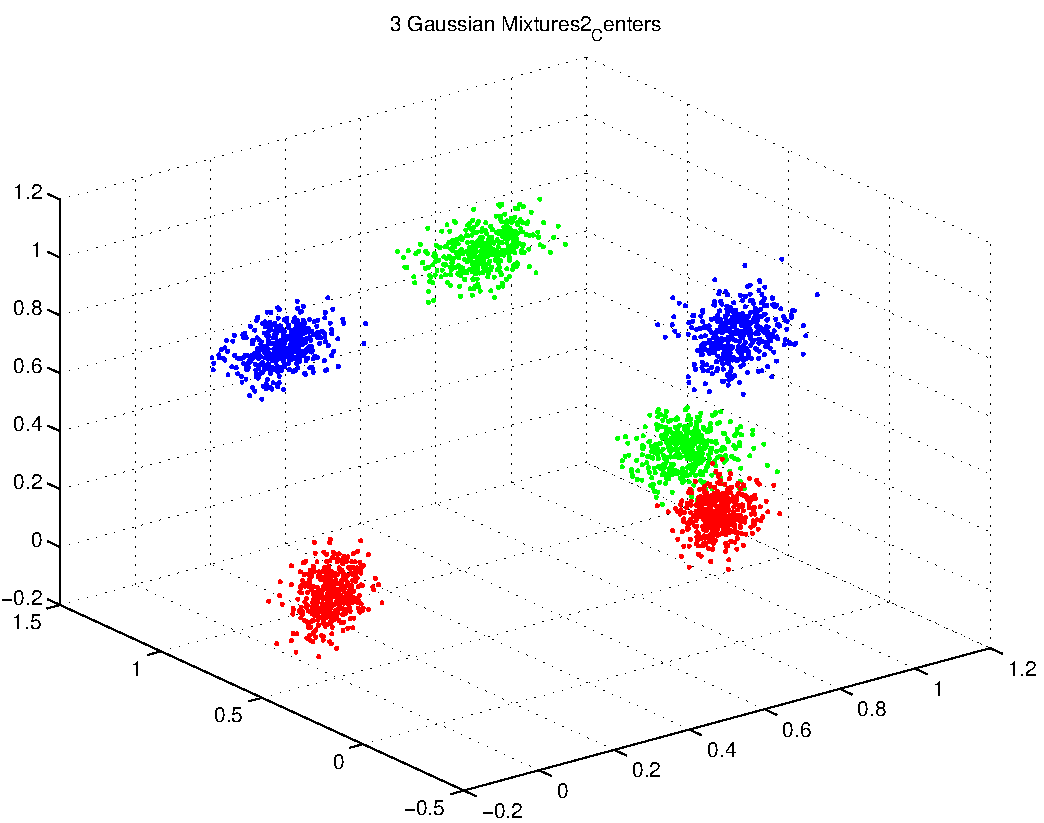
\includegraphics[width=10.0cm,height=10.0cm]{GaussianMixture_Dim_3_Centers2.pdf}

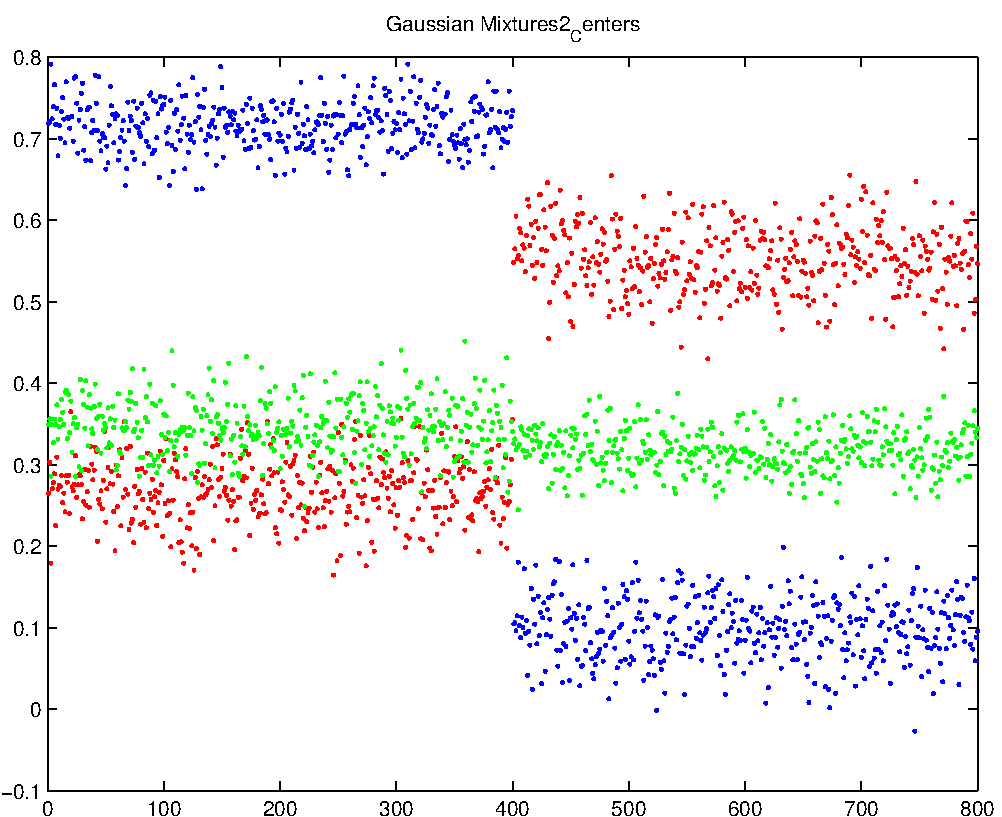
\includegraphics[width=10.0cm,height=10.0cm]{GaussianMixture_Dim_1_Centers2.pdf}

QueryPerformanceCounter  =  2.13535
\subsubsection{Matrix Quick Check <double>}
QueryPerformanceCounter  =  0.930248
\subsubsection{Matrix Quick Check <float>}
QueryPerformanceCounter  =  0.600533
\subsubsection{Intel VSL Function Check}
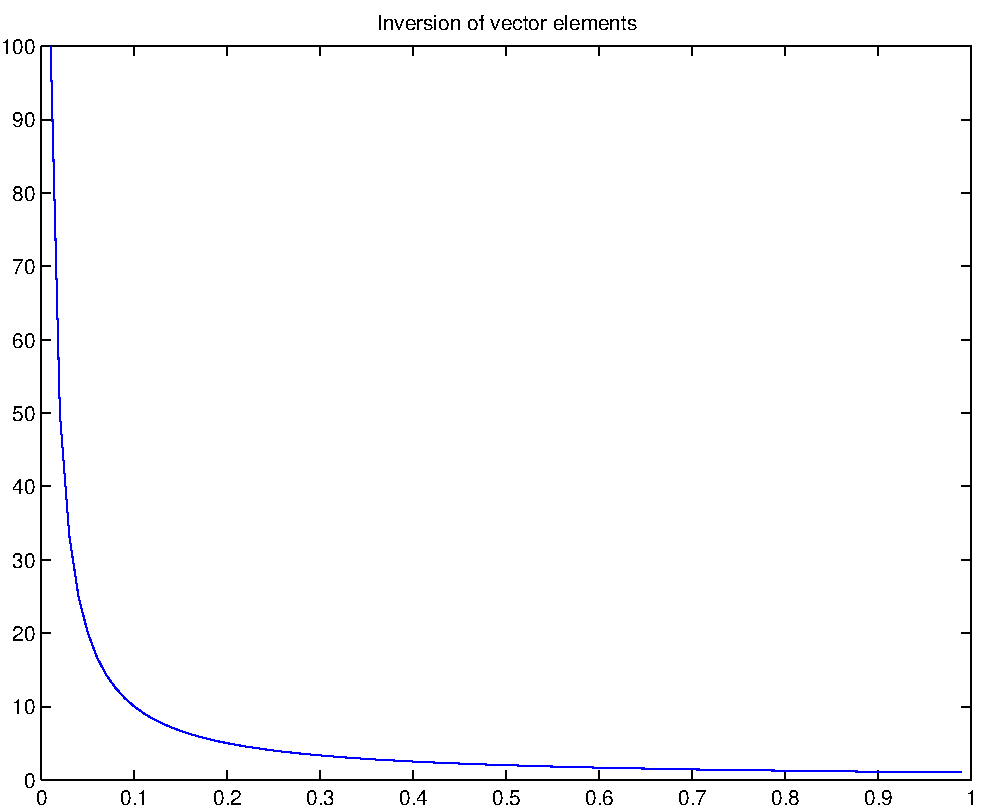
\includegraphics[width=10.0cm,height=10.0cm]{klVSLInv.pdf}

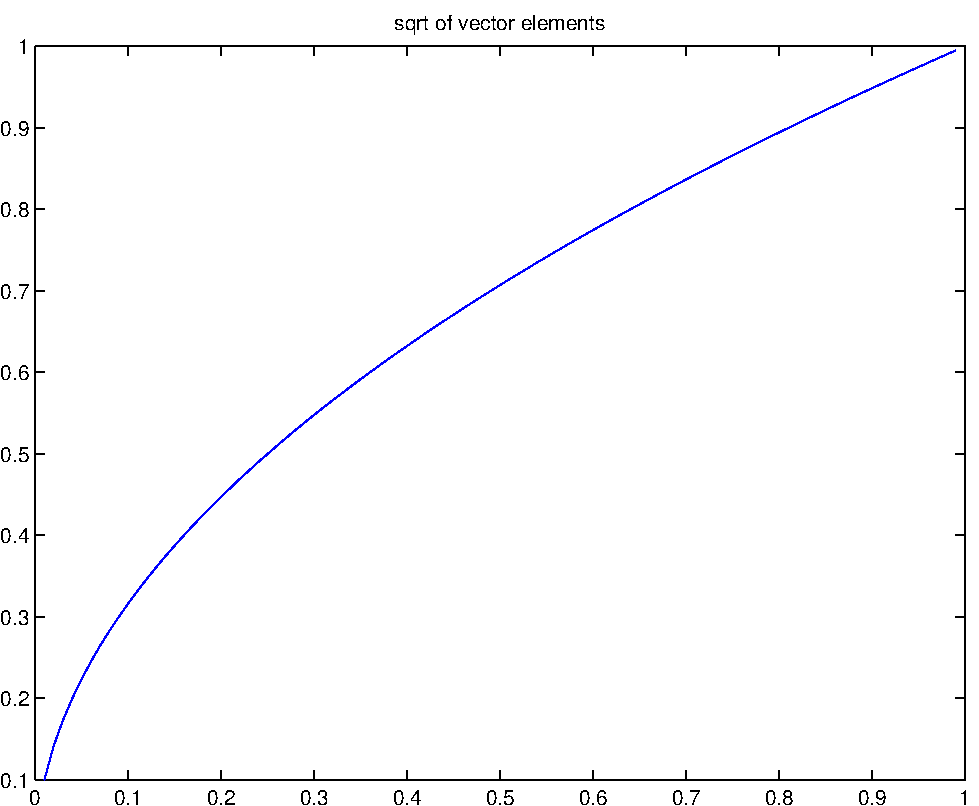
\includegraphics[width=10.0cm,height=10.0cm]{klVSLSqrt.pdf}

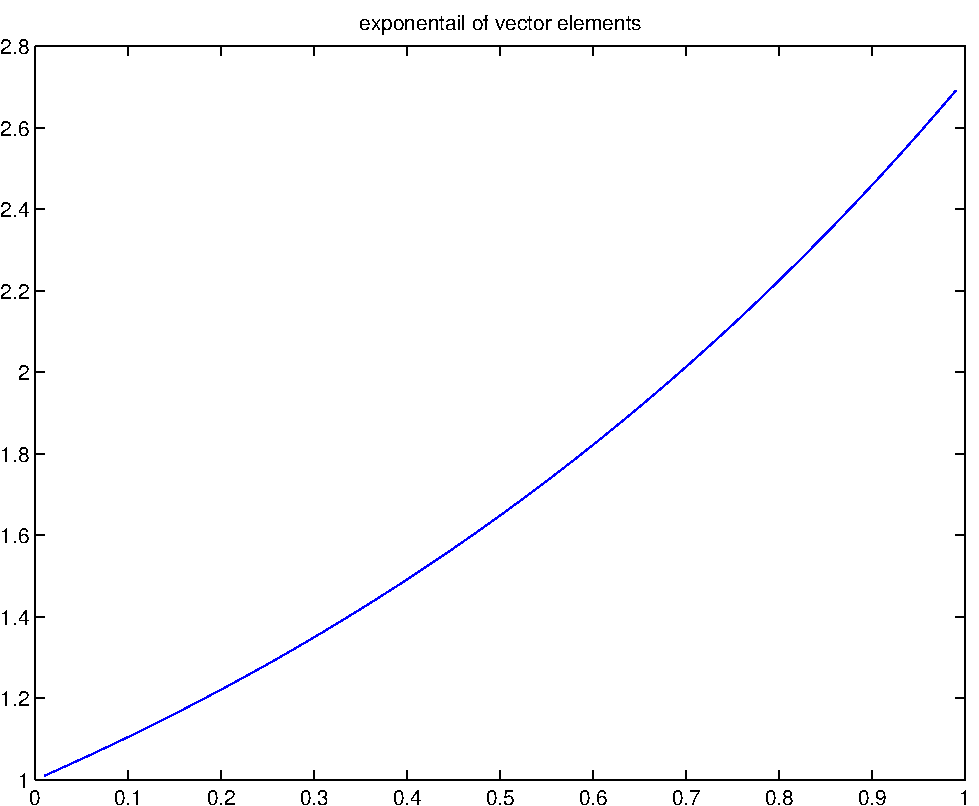
\includegraphics[width=10.0cm,height=10.0cm]{klVSLExp.pdf}

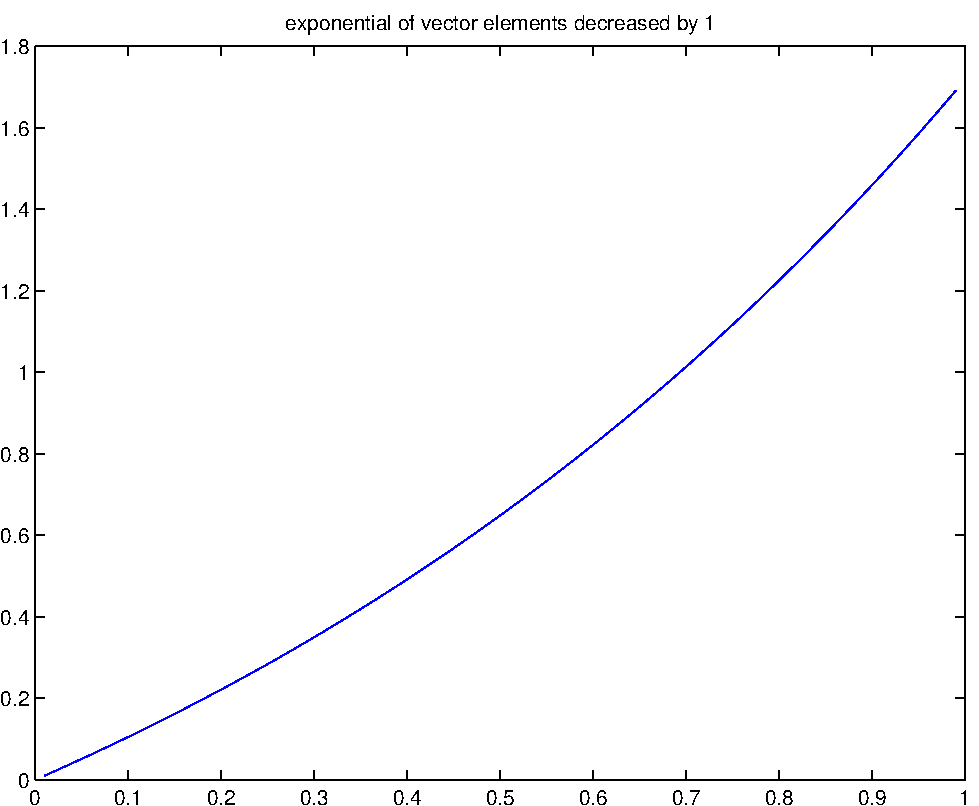
\includegraphics[width=10.0cm,height=10.0cm]{klVSLExpm1.pdf}

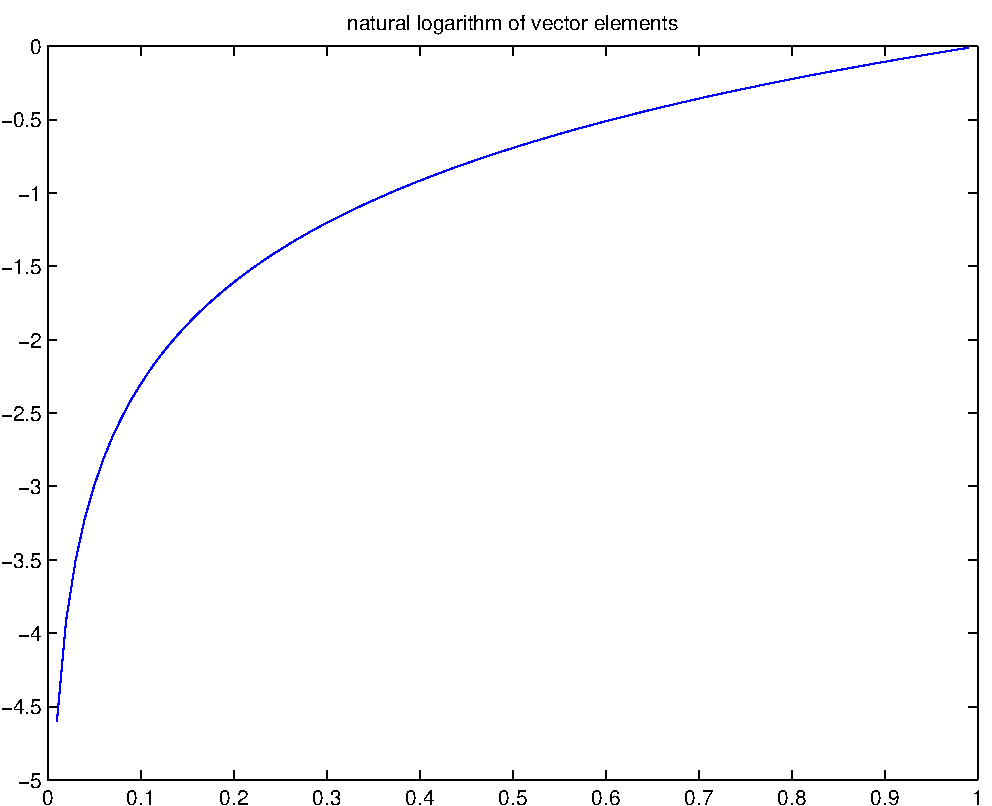
\includegraphics[width=10.0cm,height=10.0cm]{klVSLLn.pdf}

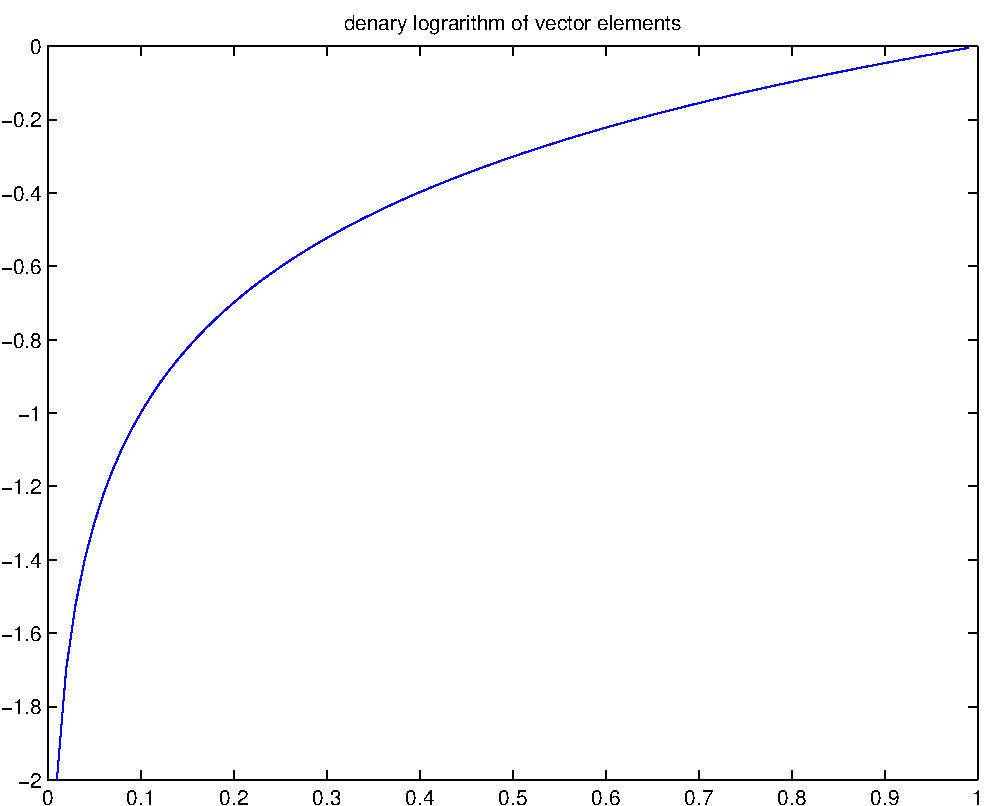
\includegraphics[width=10.0cm,height=10.0cm]{klVSLLog10.pdf}

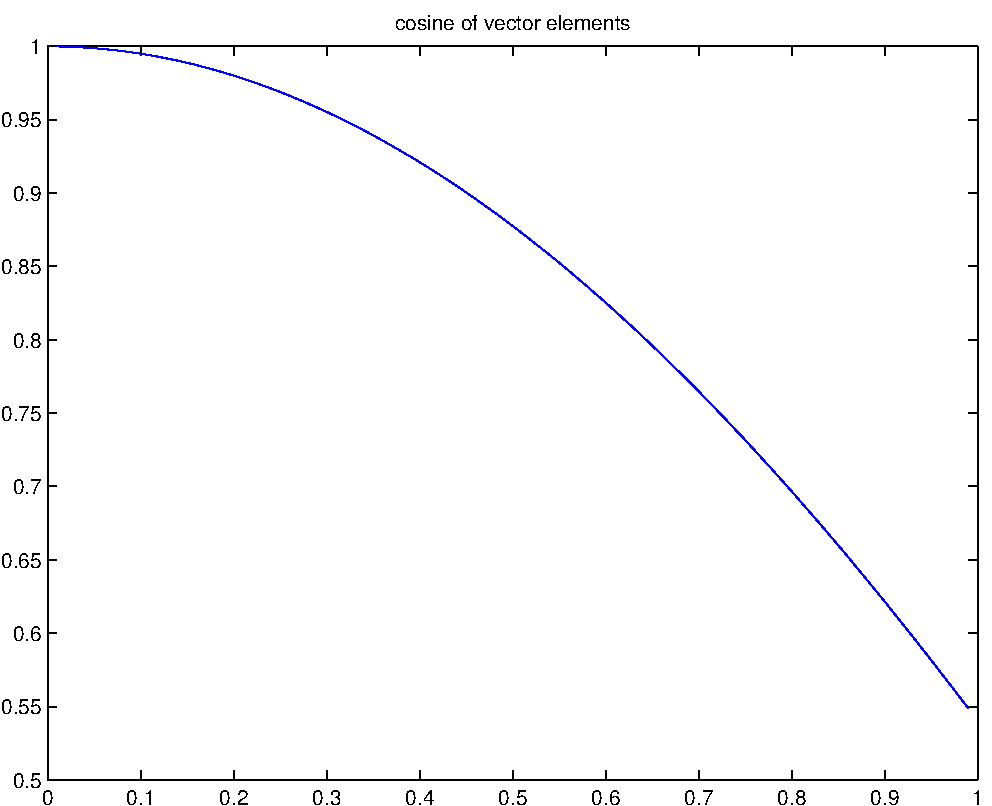
\includegraphics[width=10.0cm,height=10.0cm]{klVSLCos.pdf}

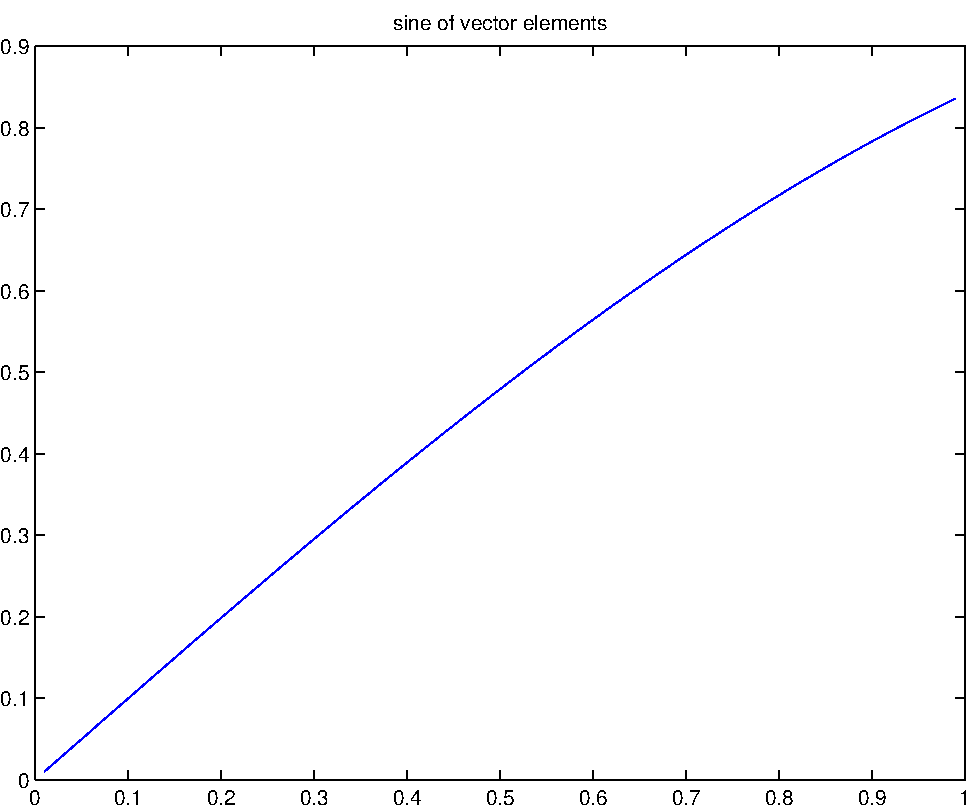
\includegraphics[width=10.0cm,height=10.0cm]{klVSLSin.pdf}

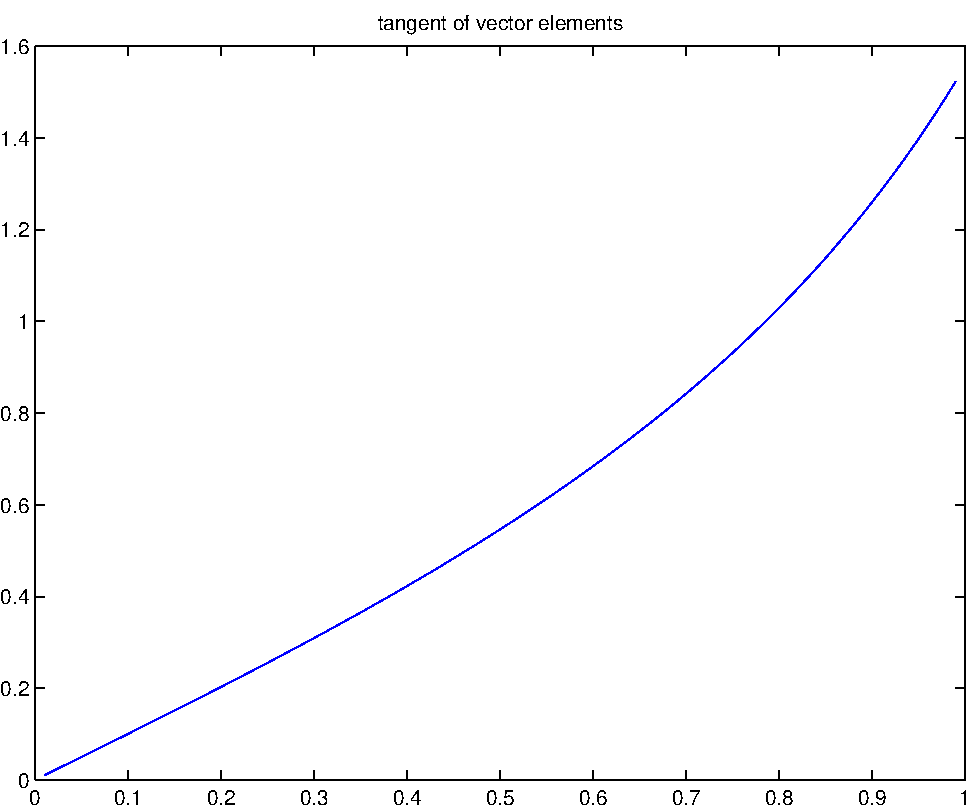
\includegraphics[width=10.0cm,height=10.0cm]{klVSLTan.pdf}

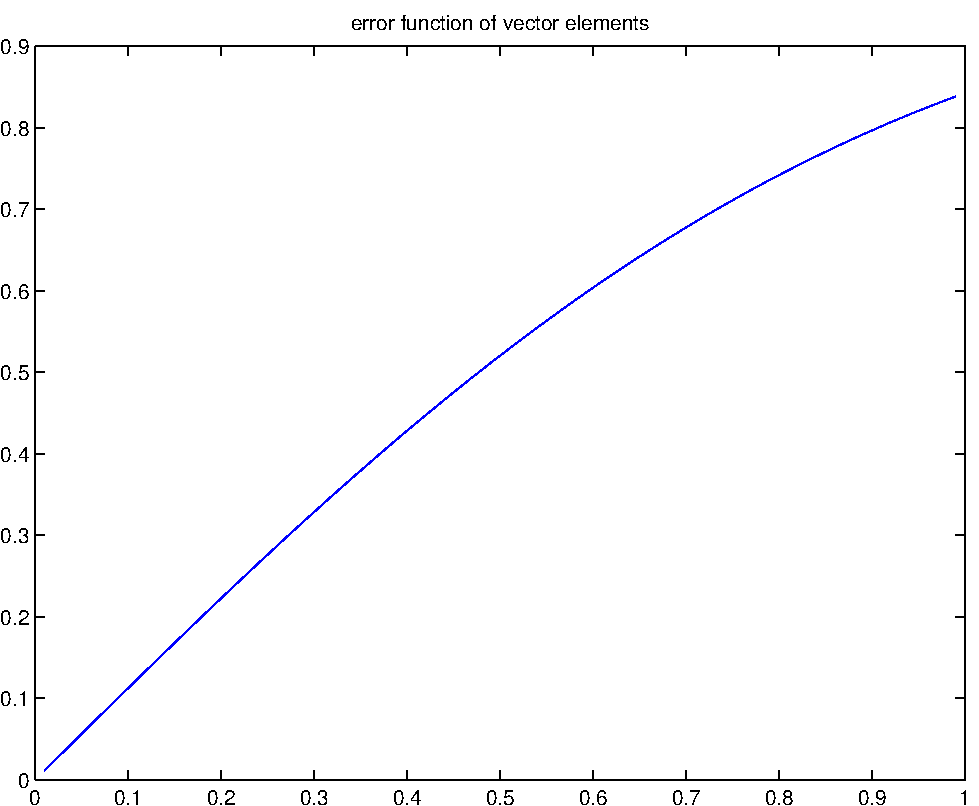
\includegraphics[width=10.0cm,height=10.0cm]{klVSLErf.pdf}

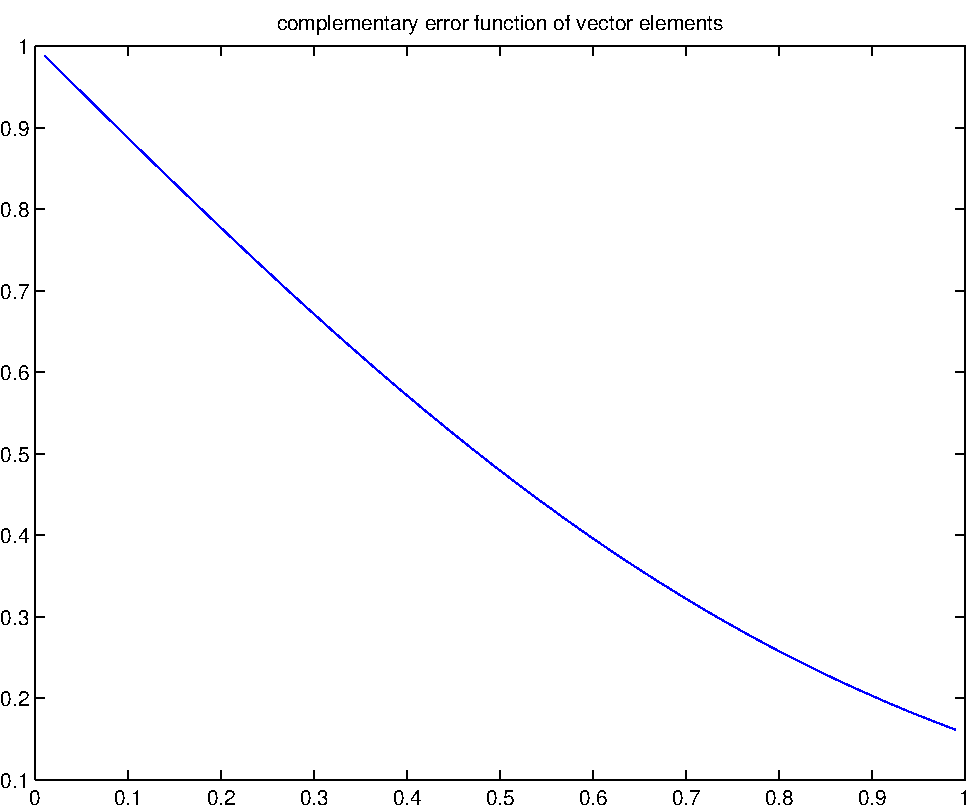
\includegraphics[width=10.0cm,height=10.0cm]{klVSLErfc.pdf}

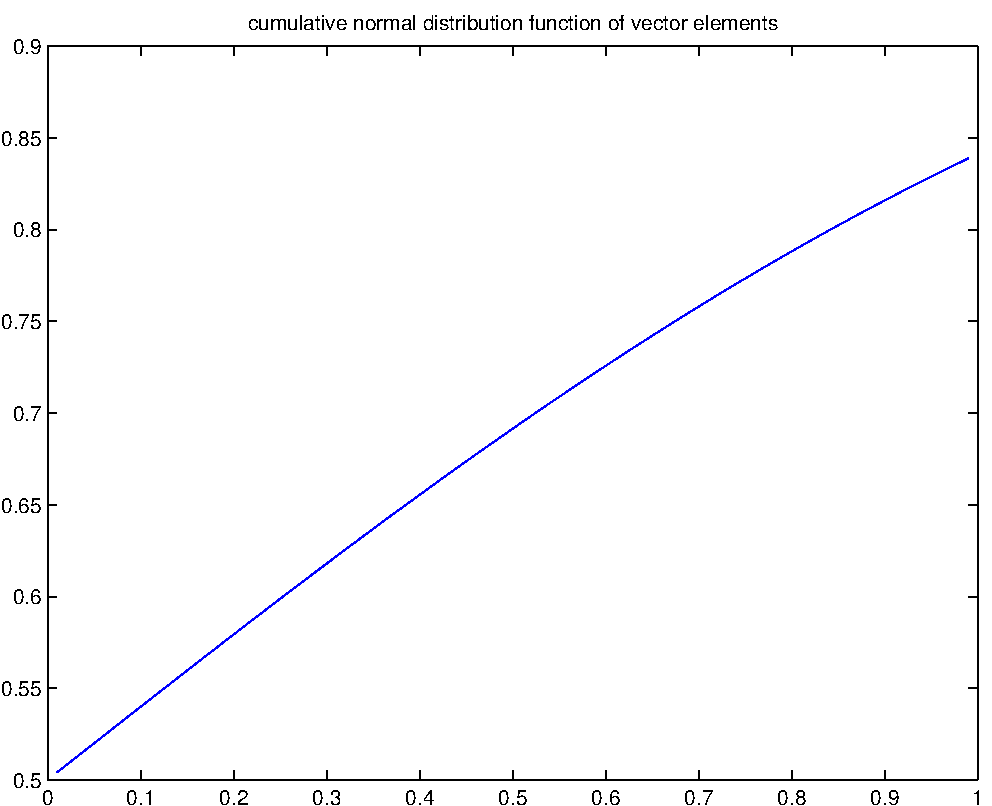
\includegraphics[width=10.0cm,height=10.0cm]{klVSLCdfNorm.pdf}

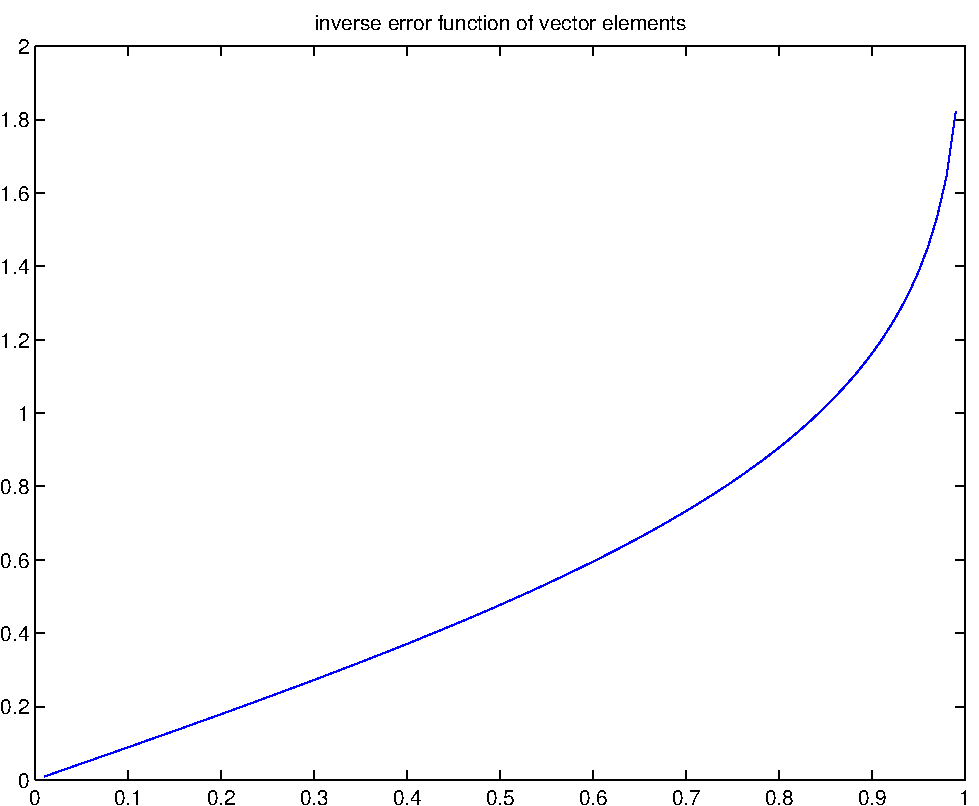
\includegraphics[width=10.0cm,height=10.0cm]{klVSLErfInv.pdf}

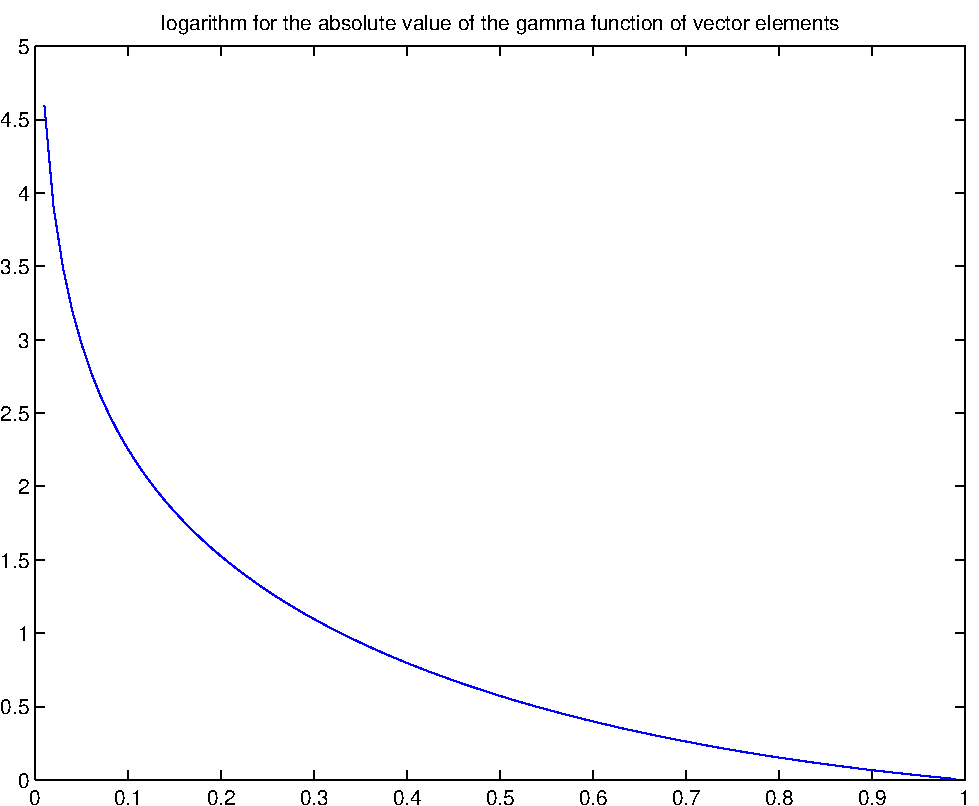
\includegraphics[width=10.0cm,height=10.0cm]{klVSLLGamma.pdf}

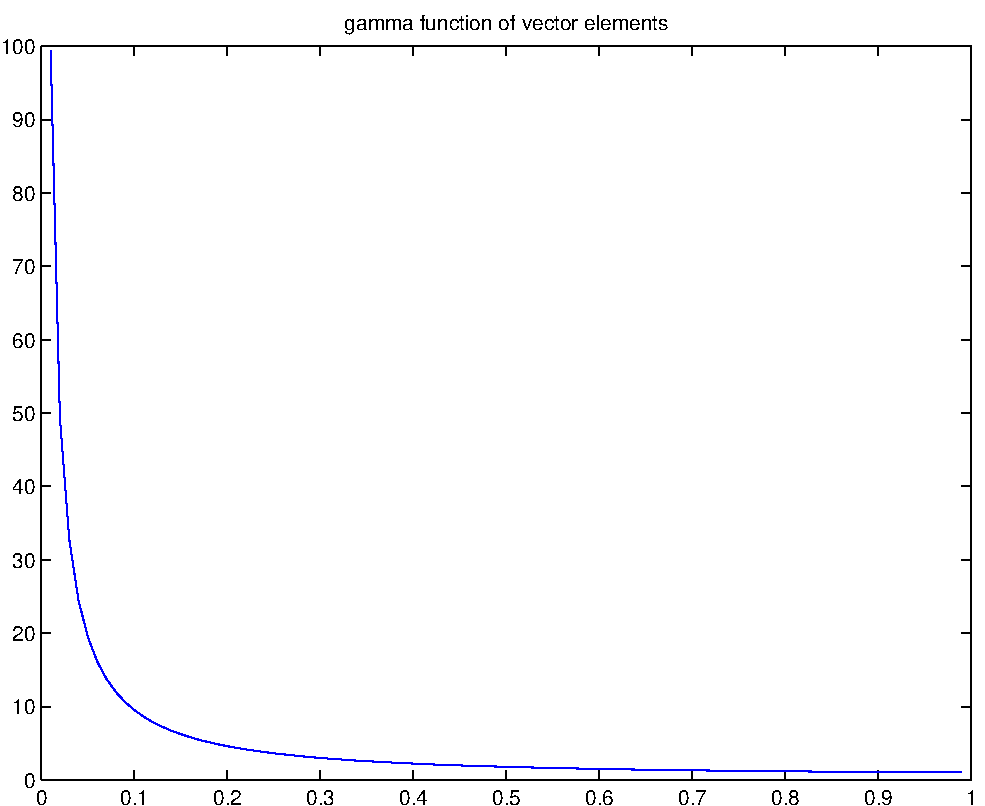
\includegraphics[width=10.0cm,height=10.0cm]{klVSLTGamma.pdf}

QueryPerformanceCounter  =  9.76096
\subsubsection{Gram Matrix Consistency Check}
Sample Size = 4096
Feature dim = 3

$$Sigma$ = \left(
\begin{array}{
ccc}
+1.140 & +1.535 & +0.581 \\
+1.535 & +9.988 & +1.605 \\
+0.581 & +1.605 & +0.428 \\
\end{array}
\right)$ \newline 

$Sample Covariance = \left(
\begin{array}{
ccc}
+1.149 & +1.489 & +0.582 \\
+1.489 & +9.975 & +1.605 \\
+0.582 & +1.605 & +0.431 \\
\end{array}
\right)$ \newline 

$Sample Mean = \left(
\begin{array}{
ccc}
+0.99291 & +0.98280 & +0.99458 \\
\end{array}
\right)$ \newline 

$Sample Covariance-$Omega$ = \left(
\begin{array}{
ccc}
+0.009 & -0.046 & +0.000 \\
-0.046 & -0.013 & -0.001 \\
+0.000 & -0.001 & +0.004 \\
\end{array}
\right)$ \newline 

$Sample Covariance Eigs = \left(
\begin{array}{
ccc}
(+10.49962,+0.00000) & (+1.01525,+0.00000) & (+0.04072,+0.00000) \\
\end{array}
\right)$ \newline 

